%%%%%%%%%%%%%%%%%%%%%%%%%%%%%%%%%%%%%%%%%%%%%%%%%%%%%%%%%%%%%%%%%%%%%%%%%%%%%%%%%%%%%%%
%%%%%%%%%%%%%%%%%%%%%%%%%%%%%%%%%%%%%%%%%%%%%%%%%%%%%%%%%%%%%%%%%%%%%%%%%%%%%%%%%%%%%%%
% 
% This top part of the document is called the 'preamble'.  Modify it with caution!
%
% The real document starts below where it says 'The main document starts here'.

\documentclass[12pt]{article}
\usepackage{graphicx}
\usepackage{float}
\usepackage{amssymb,amsmath,amsthm}
\usepackage[top=1in, bottom=1in, left=1.25in, right=1.25in]{geometry}
\usepackage{fancyhdr}
\usepackage{enumerate}
\usepackage{listings}
% Comment the following line to use TeX's default font of Computer Modern.
\usepackage{times,txfonts}

\newtheoremstyle{homework}% name of the style to be used
  {18pt}% measure of space to leave above the theorem. E.g.: 3pt
  {12pt}% measure of space to leave below the theorem. E.g.: 3pt
  {}% name of font to use in the body of the theorem
  {}% measure of space to indent
  {\bfseries}% name of head font
  {:}% punctuation between head and body
  {2ex}% space after theorem head; " " = normal interword space
  {}% Manually specify head
\theoremstyle{homework} 

% Set up an Exercise environment and a Solution label.
\newtheorem*{exercisecore}{Exercise \@currentlabel}
\newenvironment{exercise}[1]
{\def\@currentlabel{#1}\exercisecore}
{\endexercisecore}

\newcommand{\localhead}[1]{\par\smallskip\noindent\textbf{#1}\nobreak\\}%
\newcommand\solution{\localhead{Solution:}}

%%%%%%%%%%%%%%%%%%%%%%%%%%%%%%%%%%%%%%%%%%%%%%%%%%%%%%%%%%%%%%%%%%%%%%%%
%
% Stuff for getting the name/document date/title across the header
\makeatletter
\RequirePackage{fancyhdr}
\pagestyle{fancy}
\fancyfoot[C]{\ifnum \value{page} > 1\relax\thepage\fi}
\fancyhead[L]{\ifx\@doclabel\@empty\else\@doclabel\fi}
\fancyhead[C]{\ifx\@docdate\@empty\else\@docdate\fi}
\fancyhead[R]{\ifx\@docauthor\@empty\else\@docauthor\fi}
\headheight 15pt

\def\doclabel#1{\gdef\@doclabel{#1}}
\doclabel{Use {\tt\textbackslash doclabel\{MY LABEL\}}.}
\def\docdate#1{\gdef\@docdate{#1}}
\docdate{Use {\tt\textbackslash docdate\{MY DATE\}}.}
\def\docauthor#1{\gdef\@docauthor{#1}}
\docauthor{Use {\tt\textbackslash docauthor\{MY NAME\}}.}
\makeatother

% Shortcuts for blackboard bold number sets (reals, integers, etc.)
\newcommand{\Reals}{\ensuremath{\mathbb R}}
\newcommand{\Nats}{\ensuremath{\mathbb N}}
\newcommand{\Ints}{\ensuremath{\mathbb Z}}
\newcommand{\Rats}{\ensuremath{\mathbb Q}}
\newcommand{\Cplx}{\ensuremath{\mathbb C}}
%% Some equivalents that some people may prefer.
\let\RR\Reals
\let\NN\Nats
\let\II\Ints
\let\CC\Cplx

%%%%%%%%%%%%%%%%%%%%%%%%%%%%%%%%%%%%%%%%%%%%%%%%%%%%%%%%%%%%%%%%%%%%%%%%%%%%%%%%%%%%%%%
%%%%%%%%%%%%%%%%%%%%%%%%%%%%%%%%%%%%%%%%%%%%%%%%%%%%%%%%%%%%%%%%%%%%%%%%%%%%%%%%%%%%%%%
% 
% The main document start here.

% The following commands set up the material that appears in the header.
\doclabel{Stat 300: Project}
\docauthor{Stefano Fochesatto}
\docdate{\today}

\begin{document}

 In numerical analysis we are often tasked to derive well-behaved and efficiently computed 
approximations to complex mathematical functions often times in the form of a polynomial. This idea of polynomial interpolation, at it's most basic form
we encounter an interesting problem known as Runge's Phenomenon. The following is called the Runge function,
\begin{equation*}
  f(x) = \dfrac{1}{1 + 25x^2}.
\end{equation*}  
Now consider the following degree $n$ polynomial interpolants, $P_n(x)$ on the interval $[-1,1]$ with $n+1$ equally spaced points. 
\begin{figure}[H]
  \caption{Demonstration of Runge's Phenomenon}
  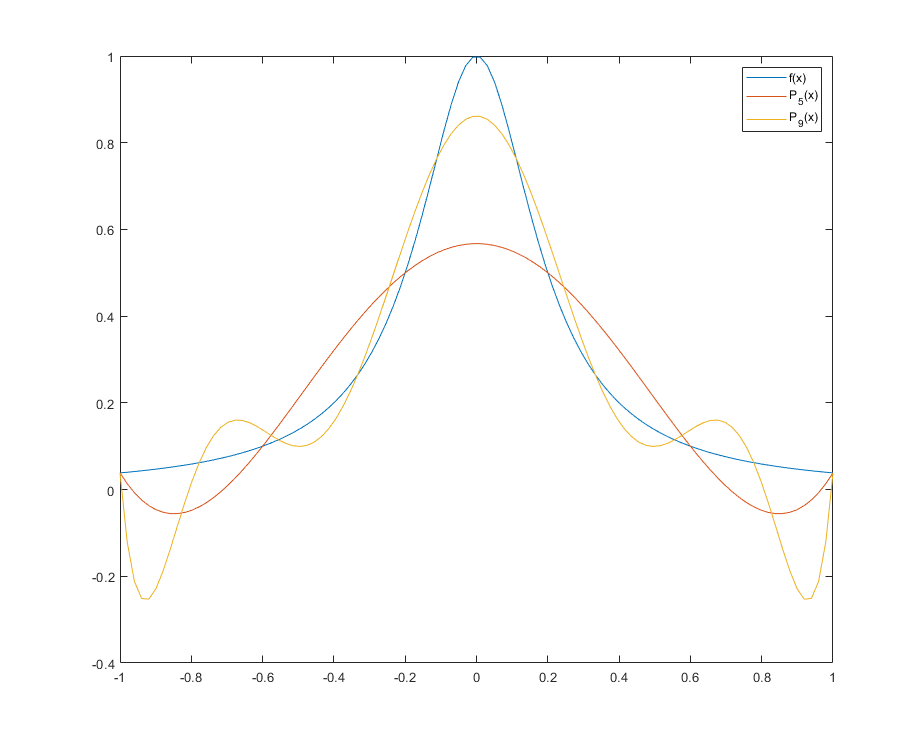
\includegraphics[width = \textwidth]{runge_example.png}  
  \centering
\end{figure}
We can see that as we interpolate our function $f(x)$ with larger and larger polynomials the oscillation at the end of 
the interval increases, and at the extremes it is a well known result that the interpolation error diverges as the degree
of the polynomial increases. Luckily there are many ways to mitigate this problem, and the method of interest as it pertains to this project is 
using Chebyshev interpolation points or (Gauss-Lobatto points). \\

 A set of $n+1$ Chebyshev points can be described with the following function, 
 \begin{equation*}
   x_i = cos(\dfrac{\pi i}{n}), i = 0, 1, \dots, n.
 \end{equation*}
 Plotting these points, we can see that they are more densely distributed towards the edges of the interval, and we can also see that
 interpolating a polynomial on these points diminished the error we saw previously with equally spaced points.


 \begin{figure}[H]
  \caption{Demonstration of Chebyshev Sampling on Polynomial Interpolation}
  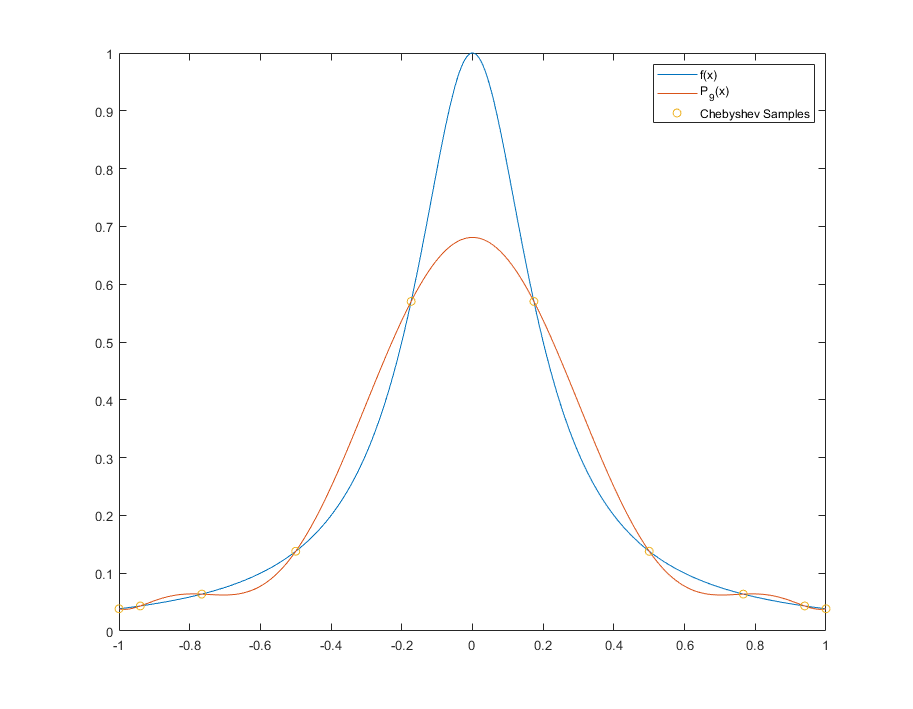
\includegraphics[width = \textwidth]{Chebyexample.png}  
  \centering
\end{figure}



 For this project we will be exploring how these points might effect the statistical accuracy of a simple linear regression, comparing them to 
 sampling data taken at evenly spaced points. To begin comparing these two sampling methods we must first simulate a data set that actually contains samples at 
 the desired sample points. Consider the following MATLAB code,  \\
 \textbf{Function:}
 \begin{center}
 \lstinputlisting{gen_data.m}
 \end{center}
 When we pass, $f(x) = x$, $a = -20$, $b = -20$, and $n = 10$ this MATLAB code generates a data set similar to the following, 
 \begin{figure}[H]
  \caption{Example of Generated DataSet}
  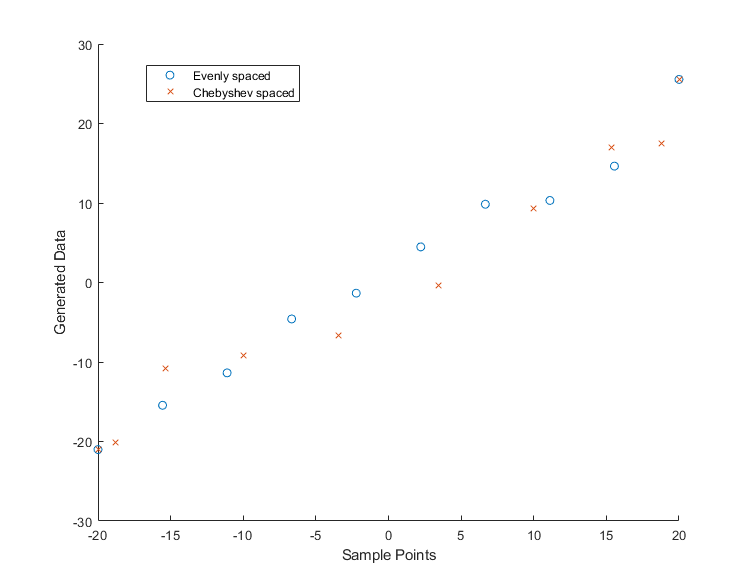
\includegraphics[width = \textwidth]{Example_generated_data.png}  
  \centering
\end{figure}

From here we can simply fit a simple linear regression to both sample sets and start our analysis of the key differences. The following MATLAB code
will fit a linear model and returns a struct with all the necessary information, similarly to the  $lm$ function in r.\\\\
\textbf{Console:}
\begin{center}
\lstinputlisting{reg.txt}
\end{center}

\begin{figure}[H]
  \caption{Example of Generated DataSet}
  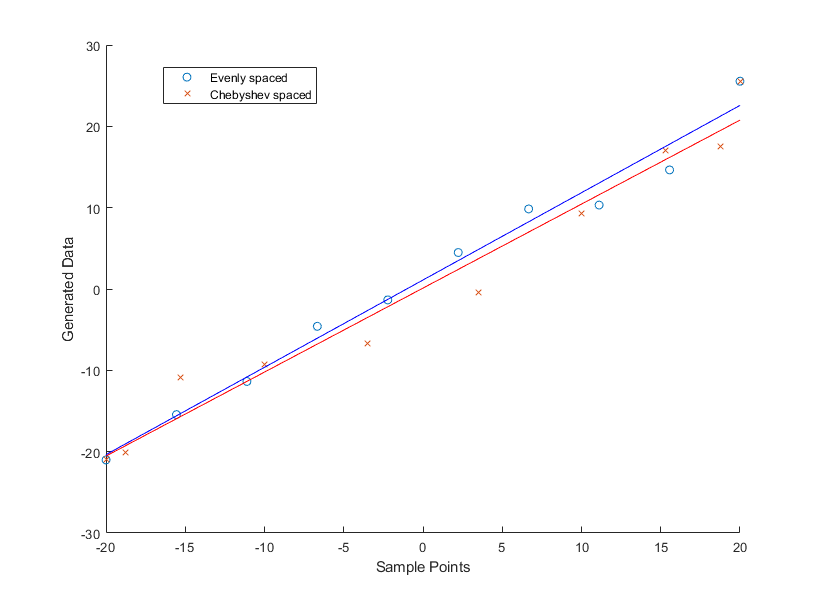
\includegraphics[width = \textwidth]{Example_generated_data2.png}  
  \centering
\end{figure}



For the analysis we conducted the same experiment 100 times with 15 sample points for each sample method, on an interval from $[-20,20]$. To see if on average there is a meaningful difference between the sampling procedure, we conducted paired sample t-test on 
goodness of fit metrics like the correlation coefficients, standard errors, and the Root Mean Square Errors. Before we get to the results let's first discuss the assumptions of a paired t-test. To conduct a paired t-test the data must be continuous, 
the data, must also be approximatly normally distributed, and finally the sample of pairs must be a simple random sample. In the case of our data all these conditions apply, and the only rule that is slightly bent is that the 
data follows a normal distribution, however with a sample size of 100 the central limit theorem kicks in and forces the sample mean of our goodness of fit variables close to normal. 
\\\\

  Looking at our findings the paired t-test showed that there was a significant statistical difference in the mean value of the Coefficient of determination. The following is a plot of 
  each $r^2$ value for each sampling method along with the results of the paired t-test.\\ 
  \begin{figure}[H]
    \caption{Plot of $r^2$ Data}
    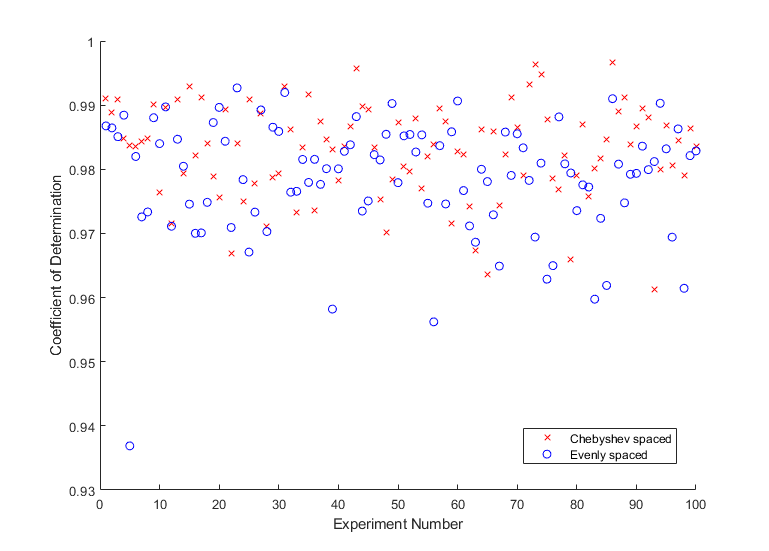
\includegraphics[width = \textwidth]{r2_data.png}  
    \centering
  \end{figure}
  \textbf{Console:}
  \begin{center}
  \lstinputlisting{r2.txt}
  \end{center}
  
  From the plot of our data there is a somewhat larger concentration of Chebyshev pints towards the top of the scatter plot and some outliers 
  for the evenly spaced points towards the bottom. With a $95\%$ confidence interval that the mean of the difference between $r^2$ values is between $(-0.00654, -0.00216)$
  its hard to justify that there is any meaningful difference between the two sampling methods with respect to $r^2$. 
  \\\\

  Looking at our data for standard error, the paired t-test also showed that there was a significant statistical difference in the mean value of the Standard Error. The following is a plot of 
  each standard error value for each sampling method along with the results of the paired t-test.\\ 
  \begin{figure}[H]
    \caption{Plot of $Standard Error$ Data}
    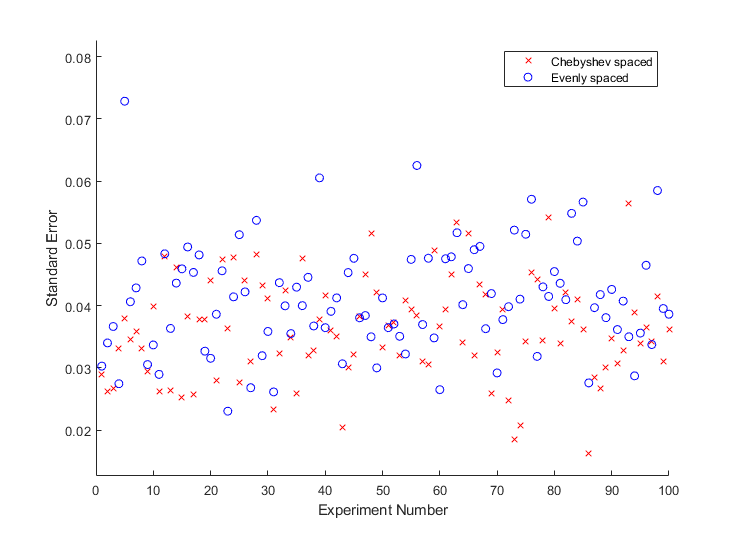
\includegraphics[width = \textwidth]{stderror.png}  
    \centering
  \end{figure}
  \textbf{Console:}
  \begin{center}
  \lstinputlisting{stderror.txt}
  \end{center}

  We an see from the plot of our data that there are around seven experiment where the evenly space sampling gave the linear model
  a somewhat larger standard error. At between experiments 70 to 100 there is a small cluster of chebyshev spaced linear models that achieved
  lower than expected standard error. Again however our paired t-test showed that on average the difference between the two standard errors, with a 
  $95\%$ confidence interval is between $(0.00266, 0.00696)$. Given that the difference is so small, I could see it being hard to justify a meaningful difference
  between the two sample methods with respect to standard error. \\\\



  Looking at our data for Root Mean Squared Error the paired t-test showed there was no significant statistical difference in the mean value of the Root Mean Square Error. The following is a plot of 
  each Root Mean Square Error value for each sampling method along with the results of the paired t-test.\\ 
  \begin{figure}[H]
    \caption{Plot of $Root Mean Square Error$ Data}
    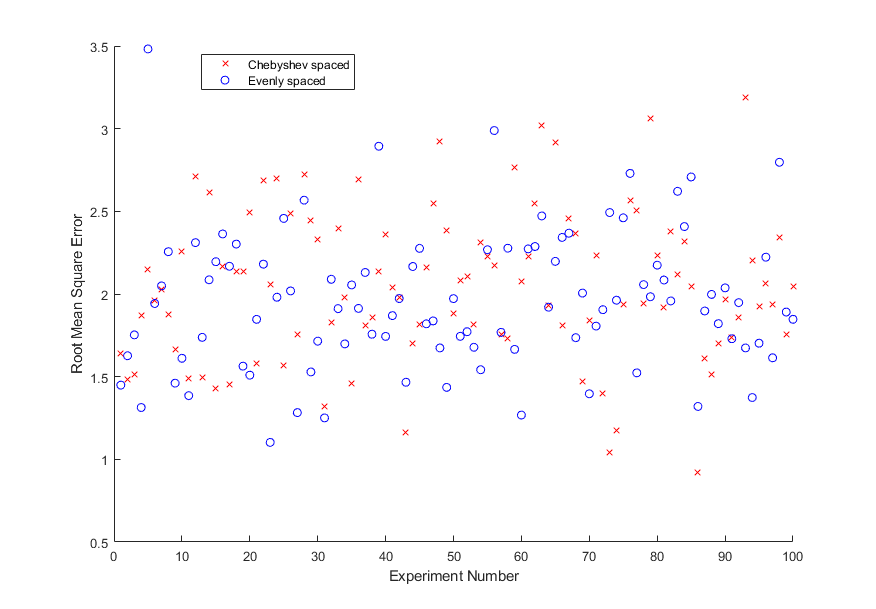
\includegraphics[width = \textwidth]{RMSE.png}  
    \centering
  \end{figure}
  \textbf{Console:}
  \begin{center}
  \lstinputlisting{RMSE.txt}
  \end{center}

  To conclude I think our finding show that in regards to some metrics it can be marginally beneficial to use a chebyshev sampling method. I took on the idea for this project after our discussion of linear models. 
  Interested in how chebyshev sampling seems to effect interpolation I figured it might be interesting to see how it would affect regression. Surprisingly from the results of this project it does seem to have a
  difference, albeit a miniscule one on the accuracy of our regressions. \\\\
  
  \newpage

  The rest of this document contains all the relevant code used throughout this project. 
  \textbf{Function:}
  \begin{center}
  \lstinputlisting{chebypoint.m}
  \end{center}
  
  \newpage
  \textbf{Function:}
  \begin{center}
  \lstinputlisting{gen_data_function.m}
  \end{center}

  \newpage
  \textbf{Function:}
  \begin{center}
  \lstinputlisting{GenerateSampleData.m}
  \end{center}











\end{document}